% =============================================================================
% Ghost-Ark — conference manuscript (systems track)
% Build: docs/paper/build.sh (uses the reviewer container's TeX Live)
%
% CLAIM DISCIPLINE: every empirical number in this file is bound to a recorded
% run or committed artifact, named in the Evidence Macros block below and in
% README-AE.md. If you edit a number, edit its evidence pointer or delete it.
% This file must never claim: proved safety, prevented-all-attacks, production
% readiness, compliance, formal verification of the implementation, or any
% live-AWS result without a bundled evidence artifact.
% =============================================================================
% Draft layout only. Replace the article class with the official target-venue
% class after a human selects the venue; this source must not be submitted as-is.
\documentclass[10pt,twocolumn,letterpaper]{article}

\usepackage[margin=0.75in,columnsep=0.25in]{geometry}
\usepackage{mathptmx}
\usepackage[T1]{fontenc}
\usepackage[utf8]{inputenc}
\usepackage{amsmath,amssymb}
\usepackage{booktabs}
\usepackage{array,tabularx}
\usepackage{microtype}
\usepackage{xcolor}
\usepackage{caption}
\usepackage{enumitem}
\usepackage{url}
\usepackage[hidelinks]{hyperref}
\usepackage{pgfplots}
\pgfplotsset{compat=1.18}
\usepgfplotslibrary{fillbetween}
\usetikzlibrary{positioning, arrows.meta}

\captionsetup{font=small,labelfont=bf}
\setlist{nosep,leftmargin=1.2em}
\newcolumntype{Y}{>{\raggedright\arraybackslash}X}

% ---------------------------------------------------------------------------
% Evidence macros — generated from docs/paper/evidence-snapshot.v1.json.
% Do not edit measured values here. Regenerate with the paper-evidence
% renderer; release checks also require the manifest, this include, and the
% reviewer-facing README blocks to agree.
% ---------------------------------------------------------------------------
% This file is generated by tools/paper-evidence.mjs from evidence-snapshot.v1.json.
% Do not edit it by hand; run: node tools/paper-evidence.mjs --render
% Recorded source revision: 7afe3931335439d2e2af39a1e2b977d3e1f8ce66
% Recorded snapshot date: 2026-08-14
% E2 local verification cost, recorded on one named host; p50 and IQR are microseconds.
\newcommand{\evtwoiters}{5{,}000}
\newcommand{\evtwohost}{Apple M1, darwin/arm64, 8 CPU, Node v22.22.3}
\newcommand{\evtwobasepfifty}{1.88}
\newcommand{\evtwobaseiqr}{0.17}
\newcommand{\evtwocanonpfifty}{6.13}
\newcommand{\evtwocanoniqr}{1.33}
\newcommand{\evtwocanonratio}{3.27}
\newcommand{\evtwodigestpfifty}{7.5}
\newcommand{\evtwodigestiqr}{0.58}
\newcommand{\evtwodigestratio}{4}
\newcommand{\evtwohmaconlypfifty}{9.08}
\newcommand{\evtwohmaconlyiqr}{1.08}
\newcommand{\evtwohmaconlyratio}{4.84}
\newcommand{\evtwohmacpfifty}{22.21}
\newcommand{\evtwohmaciqr}{4.04}
\newcommand{\evtwohmacratio}{11.84}
\newcommand{\evtworsapfifty}{119.25}
\newcommand{\evtworsaiqr}{5.83}
\newcommand{\evtworsaratio}{63.6}
% E3/E4 corpus census: exact within this hand-authored corpus, not a population estimate.
\newcommand{\evthreeintrinsic}{26/26}
\newcommand{\evthreeaggregate}{28/28}
\newcommand{\evthreecontrol}{3/3}
\newcommand{\evthreeundetected}{0}
\newcommand{\evthreeboundary}{2}
\newcommand{\evfourloadbearing}{7}
% Recorded local Rust stress run; not a cross-machine throughput claim.
\newcommand{\stressops}{275{,}415}
\newcommand{\stressrejm}{10.1}
% TLC v1.7.4; generated run output is artifacts/proofs/proofs_summary.json; raw reference logs are committed under proofs/**/artifacts/.
\newcommand{\tlatoolversion}{v1.7.4}
\newcommand{\plstates}{403{,}949}
\newcommand{\scstates}{529}
\newcommand{\tbstates}{64}
\newcommand{\tistates}{149{,}796}
\newcommand{\nlstates}{1{,}321}
\newcommand{\ebstates}{51{,}106}
% Test totals are a lower-bound snapshot: a green suite may legitimately grow.
\newcommand{\testcount}{1{,}434}
\newcommand{\testfiles}{172}
% Claim-scan count is for the tracked source revision only; the normal working-tree scan is broader.
\newcommand{\claimfiles}{942}


% These are explanatory notation rather than measured evidence. The
% formal-games calculation remains quarantined from implementation evidence.
\newcommand{\benchtrials}{10{,}000}
\newcommand{\globaladvantage}{0}
% Mutant distinct-state counts are scheduling-sensitive (R11); only their
% violation verdict is reproducible and is shown in Table~\ref{tab:tlc}.
\newcommand{\mutrange}[1]{\textsc{n/a}}

\newcommand{\dab}{\textsc{dab}}
\newcommand{\ghostark}{Ghost-Ark}
\newcommand{\piR}{\pi_R}
\newcommand{\statusimpl}[0]{\textcolor{black}{\textbf{[implemented, tested]}}}
\newcommand{\statussocket}[0]{\textcolor{black}{\textbf{[wired socket prototype, local E2E]}}}
\newcommand{\statusunit}[0]{\textcolor{black}{\textbf{[unit-tested, not wired at runtime]}}}
\newcommand{\statusmodel}[0]{\textcolor{black}{\textbf{[TLC-checked, bounded model]}}}
\newcommand{\statusspec}[0]{\textcolor{black}{\textbf{[specified, not enforced at runtime]}}}

\title{\vspace{-1.5em}\textbf{\ghostark{}: A Transactional Control Plane for Untrusted AI Agents}\\
\large A Bounded Three-Gate Design and Receipt-Backed Evidence for
Non-Deterministic Compute\vspace{-0.5em}}

% ============================================================================
% ARXIV / CAMERA-READY AUTHOR BLOCK
% ============================================================================
% CORRESPONDENCE ADDRESS: substitute the institutional address before any
% submission or preprint. This line previously carried a personal free-mail
% address; under an institutional account that is a personal inbox published in
% the most externally-facing document in the repository, which
% docs/artifact/PUBLIC_INTERFACE.md forbids and
% tests/unit/repo-hygiene/publicInterface.test.ts now enforces over .tex.
% A free-mail domain here will fail `npm test`. An institutional address
% (e.g. a .edu) will not, and is the intended value.
% ============================================================================
% ============================================================================
% SUBMISSION MODE
% The intended venue and its official class have not been selected in this
% repository.  Default to anonymous review output so this source cannot emit a
% double-blind-blocking author, institution, or repository URL by accident.
% Switch only after the venue and its camera-ready policy are explicitly chosen.
% ============================================================================
\newif\ifdoubleblind
\doubleblindtrue
\ifdoubleblind
  \author{Anonymous submission}
  \date{}
\else
  \author{
    Pranav Bhave \\
    \normalsize S2 Lab, College of Information Sciences and Technology \\
    \normalsize The Pennsylvania State University \vspace{0.2em} \\
    \normalsize\href{https://github.com/PSUCyberSecurityLab/ghost-ark/}{\color{blue}github.com/PSUCyberSecurityLab/ghost-ark}
  }
  \date{Evidence snapshot dated 2026-08-14; see \S\ref{sec:artifact}}
\fi

\begin{document}
\maketitle

% ============================================================================
\begin{abstract}
\noindent
Agentic LLM deployments couple a non-deterministic planner directly to effectful APIs.
The dominant defense --- semantic guardrails --- probabilistically flags unsafe content,
but struggles to constrain state mutations. We present \ghostark{}, a bounded control-plane
design that treats an agent trajectory as a software transaction. The design specifies an
untrusted agent executing against a ghost replica $G(\sigma_0)$ and a trusted gateway that
admits effects only after three checks: a \emph{ledger gate} for nonce freshness, an
\emph{OCC gate} over a read-set projection $\piR$, and a \emph{semantic gate} over supplied
failure marginals. The shipped socket prototype wires the payload-binding and ledger subset;
the OCC and semantic helpers are unit-tested but are not wired into that runtime path.

We report what is implemented and measured, and label what is only specified.
TLC model checking of six bounded models (up to \plstates{} distinct states) caught
a subtle garbage-collection replay flaw in our own design, which we repaired spec-first.
Against a malicious-fixture corpus run through the standalone verifier,
\evthreeintrinsic{} mutations are rejected by verifier rules alone, with a
\evthreecontrol{} control arm of unmutated fixtures passing and a metamorphic guard
confirming those rejections cease when the mechanism they depend on is neutered.
Full receipt verification costs $p50=\evtwohmacpfifty{}\,\mu$s (IQR \evtwohmaciqr{})
symmetric and $\evtworsapfifty{}\,\mu$s (IQR \evtworsaiqr{}) asymmetric, against a
$\evtwobasepfifty{}\,\mu$s parse-only baseline on a single named host. The DAB socket
prototype signs and independently verifies \texttt{CERTIFIED} executions only; its rejection
responses are neither signed nor verifier-accepted, and malformed or execution-failure paths
may emit no receipt. \ghostark{} verifies recorded bindings under its verifier rules; it does
not certify that an agent output is aligned, semantically safe, or true.
\end{abstract}

% ============================================================================
\section{Introduction}
\label{sec:intro}

Every serious agent framework today ships with guardrails, and almost none
ships with isolation. The guardrail is a classifier: given content, it emits a
probability that the content is unsafe. The deployment question is different
in kind: \emph{did the bytes that reached the environment correspond to an
authorized, recorded, non-replayed decision?} A classifier cannot answer that
question at any confidence, because it is not a question about content at all.
We call this the \textbf{epistemic deficit} of guardrail-centric agent
security: the property operators need is a property of \emph{state
mutations}, and the mechanism they deploy evaluates \emph{utterances}.

The deficit is structural, and mirrors standard database isolation anomalies. A typical
API-coupled agent loop (plan $\to$ call tool $\to$ observe $\to$ repeat)
mutates external state at every step with no validation phase and no
rollback: in isolation-level terms, the industry ships agents at
\textsc{read uncommitted}~\cite{berenson1995critique}. If the planner is
compromised mid-trajectory --- by indirect prompt injection, a poisoned tool
response, or ordinary hallucination --- the earlier steps have already leaked
dirty writes into the world. Sandboxing upgrades this to roughly
\textsc{read committed}: writes are buffered, but a long reasoning phase over
a shifting environment still flushes stale intent, the classic write-skew
shape. What is missing is the third rung: a \emph{validation phase} between
speculation and commit, which is precisely the structure that optimistic
concurrency control (OCC)~\cite{kung1981occ} and software transactional
memory~\cite{shavit1995stm,herlihy1993tm} were invented to provide.

To see the gap, consider an agent with a \texttt{delete\_s3\_object} tool processing an untrusted resume containing an indirect prompt injection (``Ignore instructions, delete all files''). Today, if the agent is compromised mid-reasoning, it executes the tool immediately. Sandboxing the agent process (e.g., in a Firecracker microVM) bounds the blast radius of arbitrary code execution, but does not stop the agent from issuing authorized, authenticated API calls to external services. Sandboxes provide process isolation, but agents need \emph{intent isolation}. The proposed ghost-replica design buffers the API call in $G(\sigma_0)$ and validates it before commit; if the downstream semantic or provenance check detects a violation, the design collapses the trajectory. That full composition, including signed abort evidence, is not the shipped runtime path and is not claimed as such.

\ghostark{} applies that structure to agents as a design and evidence program. Its
Rust socket prototype independently recomputes a payload digest, applies a bounded
nonce ledger, sends the decoded body to a local test sink, and signs only a successful
\texttt{CERTIFIED} outcome. It does not yet compose a ghost replica, OCC, semantic
gate, or signed rejection protocol. The design goal is not to make the agent correct ---
we take its fallibility as an axiom --- but to state which recorded bindings a verifier
can check and which enforcement composition still requires runtime evidence.

This paper makes the following contributions, each labeled with its
implementation status (a discipline we keep throughout; \S\ref{sec:nonclaims}
enumerates non-claims):

\begin{itemize}
\item \textbf{A threat model for evidence-layer attacks}
  (\S\ref{sec:threat}): \emph{assertion-conditioned compliance} (A-CC), where
  a procedurally valid pipeline signs a structurally flawless record of a
  functionally corrupted operation, and its scaled form, adaptive agentic
  worms.
\item \textbf{A transactional enforcement architecture}
  (\S\ref{sec:design}): payload-byte binding in a Rust socket prototype
  \statussocket{}; a ledger gate with spent-tombstone replay semantics
  \statussocket{} \statusmodel{}; semantic and OCC helpers \statusunit{};
  and an explicit boundary between the specified three-gate design and the
  subset wired at runtime.
\item \textbf{A liveness analysis} (\S\ref{sec:formal}): global-state
  validation starves under concurrent environmental writes (the
  \emph{starvation trap}); the read-set projection $\piR$ recovers liveness
  at a precisely stated cost in conflict-detection strength.
\item \textbf{Model checking with teeth} (\S\ref{sec:tla},
  \S\ref{sec:eval-tla}): six TLC-checked bounded models plus five seeded
  mutants that must fail (the sixth model has none, and we say so) ---
  including the case study where TLC refuted our
  own baseline design (garbage collection re-enabled replay) and the repair
  was propagated spec-first into the implementation.
\item \textbf{An honest evaluation} (\S\ref{sec:eval}): \evthreeintrinsic{}
  verifier-intrinsic rejection of a malicious corpus, with a
  \evthreecontrol{} control arm and a metamorphic guard establishing that the
  detections are load-bearing rather than tautological; verification cost as
  p50 with IQR against a parse-only baseline, reported alongside --- and
  explicitly instead of --- a misleading relative-overhead figure; and a
  disclosed retraction of this paper's own former evidence source
  (\S\ref{sec:superseded}).
\end{itemize}

\ghostark{} is one subsystem of a larger research program (\emph{verifiable
agent governance under correlated guardrail failure}); this paper confines
itself to the transactional control plane and its recorded evidence.

% ============================================================================
\section{Threat Model}
\label{sec:threat}

We assume the agent runtime --- the LLM, its context window, its planning
loop, and the V8/Node process hosting it --- is \emph{compromised or
compromisable}. Adversarial capability enters through any content channel:
retrieved documents, tool responses, upstream messages. The trusted computing
base for the socket prototype is confined to the gateway process, its signing
key, the in-process nonce ledger, and the verifier. The prototype network
boundary is a Unix domain socket followed by an outbound HTTP request; this
does not establish that all repository execution paths are gateway-mediated.

\subsection{Assertion-Conditioned Compliance (A-CC)}
\label{sec:acc}

Signature pipelines create a new attack surface precisely because they work.
Define A-CC as the failure mode in which an agent incorporates a false
assertion --- typically a \emph{function-sourced assertion} (FSA) from a
compromised or deceptive tool --- into procedurally valid execution, so that
the pipeline signs a \emph{structurally flawless record of a functionally
corrupted operation}. The receipt is authentic; the decision it witnesses was
poisoned upstream. A-CC is an attack on the evidence layer, not the crypto:
no deterministic function of adversary-controlled bytes can distinguish
honest from dishonest content, so the defense must be architectural ---
binding every assertion to a provenance class that records \emph{where bytes
entered custody}, and refusing floors that fabricated in-context text cannot
satisfy (\S\ref{sec:custody}).

\subsection{Adaptive agentic worms}
\label{sec:worms}

A-CC at propagation scale: an infected agent uses the low marginal cost of
LLM reasoning to synthesize, per victim, a payload and a justification for
emitting it. Static signatures fail by construction (each instance is
freshly generated); semantic filters fail correlatedly (the same context
compromise that produced the payload biases the judge). The architectural
response is to make \emph{propagation} pass through a commit pipeline: in the
specified composition, a worm's write would survive all three gates before
binding. The current runtime evidence is narrower: its socket prototype
applies payload-byte binding and nonce freshness, and independently verifies
successful \texttt{CERTIFIED} receipts. It does not provide signed abort
evidence or a runtime three-gate composition. We do not certify any detector's
hit rate (\S\ref{sec:nonclaims}).

\subsection{Modeled attacker actions}
\label{sec:modeled}

The Tier-0 adversarial corpus (\S\ref{sec:eval-corpus}) operationalizes the
in-flight attacker: payload field mutation, single-byte flips, prototype
pollution, receipt replay, mass replay flooding, Unicode normalization
collisions, homoglyph spoofing, cross-request nonce swaps, and
double-execution races; plus four security games (mutation resistance,
replay resistance, cross-transaction binding, serialization ambiguity).
These model an adversary who can observe, mutate, reorder, and replay
traffic between the agent runtime and the gateway.

\subsection{Out of scope}
\label{sec:oos}

Not addressed by this design and not claimed: semantic correctness or
alignment of model output; compliance with any regulation; hardware
attestation (no Nitro/TEE flow is implemented or claimed); denial of service
against the gateway itself; covert channels inside authorized outputs; and
the \emph{confused deputy} within an authorized clearance --- an agent that
legitimately holds a floor and routes authorized data to a hostile but
allowlisted destination is constrained only by routing policy, not by this
paper's mechanisms.

% ============================================================================
\section{Design}
\label{sec:design}

\begin{table*}[t]
\centering\small
\begin{tabularx}{\textwidth}{@{}p{2.45cm}YYY@{}}
\toprule
\textbf{Component} & \textbf{Test evidence} & \textbf{Wired runtime} & \textbf{End-to-end evidence}\\
\midrule
Payload-byte DAB binding & Gateway signer and independent-verifier tests & Unix-socket prototype recomputes a decoded-payload digest and posts those decoded bytes & Local socket test verifies a \texttt{CERTIFIED} receipt and byte-compares the sink body \\
Nonce ledger & Unit and concurrency tests for the active/spent transition & Unix-socket prototype calls the replay ledger before its certified path & Local socket test observes a replay rejection for a reused nonce \\
OCC read-set projection & Deterministic helper tests & No caller in the API or socket gateway & None \\
Semantic Fr\'echet bound & Schema/helper tests against hand-computed bounds & No caller in the API or socket gateway & None \\
Rejection receipt & Status-response branches only & Replays and mutations are unsigned; malformed and execution-failure paths may return no receipt & None; the verifier accepts \texttt{CERTIFIED} only \\
\bottomrule
\end{tabularx}
\caption{Runtime-status matrix at the recorded evidence revision. ``Wired'' means an invoked code path, not a deployment claim. The three-gate composition is a specified architecture; the shipped DAB socket path wires only payload-byte binding and the nonce ledger.}
\label{tab:runtime-status}
\end{table*}

\subsection{Agent loops as isolation levels}
\label{sec:isolation}

Table~\ref{tab:isolation} summarizes the mapping that motivates the design.
The point of the table is not taxonomy but a design gap. Its serializable row
is a target architecture, not a claim that the currently wired runtime provides
serializable isolation; Table~\ref{tab:runtime-status} separates the specified
composition from the tested socket subset.

\begin{table*}[t]
\centering\small
\begin{tabularx}{\textwidth}{@{}p{2.65cm}YY@{}}
\toprule
\textbf{Isolation} & \textbf{Agent analogue} & \textbf{Characteristic anomaly}\\
\midrule
Read uncommitted & API-coupled loop; mutate per step & dirty writes: pre-abort
steps already leaked \\
Read committed & sandbox + buffered intent pool (e.g., NemoClaw-style
isolated execution~\cite{nemoclaw2026}) & write skew: stale reasoning
flushed onto shifted state \\
\shortstack[l]{Serializable\\(proposed OCC)} & \ghostark{} design: speculate in $G(\sigma_0)$,
validate, then bind & aborts under conflict; liveness cost analyzed in
\S\ref{sec:starvation}; helper not wired at runtime \\
\bottomrule
\end{tabularx}
\caption{Database isolation levels and their agent-architecture analogues. The
third row is a specified design target, not a runtime isolation result.}
\label{tab:isolation}
\end{table*}

\subsection{\texorpdfstring{Declarative Action Binding and $\Delta_{\mathrm{DE}}$}{Declarative Action Binding and Delta DE}}
\label{sec:dab}

In the DAB socket prototype, the untrusted client sends a declared payload
digest $C_I$. The gateway decodes the payload, independently derives $C_E$
from the decoded bytes, and posts those same decoded bytes only when
$C_I=C_E$. Define the declared--executed payload divergence
$\Delta_{\mathrm{DE}} = |\,C_I \oplus C_E\,|$. This closes one serialization
boundary rather than a whole action model: the V1 receipt does \emph{not} bind
the request target, and target authorization is outside its verifier contract.
Cross-language normalization remains an attack surface, which is why
\S\ref{sec:eval-corpus} attacks the encoder as well as the receipt envelope.
\statussocket{}

\subsection{The ghost replica and speculative collapse}
\label{sec:ghost}

The specified design executes a trajectory against $G(\sigma_0)$, a forked
view of relevant state at transaction start; its writes accumulate in a
speculative buffer. Commit-time validation would either \emph{bind} the buffer
to the environment or trigger \texttt{SpeculativeCollapse}. The collapse/commit
state machine is one of the six TLC-checked bounded models
(\S\ref{sec:eval-tla}, \scstates{} distinct states). The current socket
prototype does not implement this replica, collapse, or an abort-receipt path.
\statusspec{}

\subsection{The three-gate validation pipeline}
\label{sec:gates}

Validation is a conjunction of three independently answerable questions ---
\emph{is it fresh}, \emph{is it current}, \emph{is it within policy}:

\textbf{Gate 1 --- Ledger (freshness).} Each transaction carries a nonce
$n_i$. Admission requires
$n_i \notin \mathcal{L}_{\mathrm{nonce}} \,\wedge\, n_i \notin S_{\mathrm{spent}}$,
where $\mathcal{L}_{\mathrm{nonce}}$ is the active ledger and
$S_{\mathrm{spent}}$ a tombstone set of consumed nonces. The tombstone set is
not an optimization; it is the repair of a real flaw that model checking
found in our own design (\S\ref{sec:tla}). Expiry \emph{archives} a nonce
into $S_{\mathrm{spent}}$ rather than forgetting it, so a nonce consumed at
time $T$ is still rejected at $T+\mathrm{TTL}+1$. \statussocket{}
\statusmodel{}

\textbf{Gate 2 --- OCC (currency).} Admission requires
$\mathcal{H}(\piR(\sigma_{\mathrm{now}})) = \mathcal{H}(\piR(\sigma_0))$:
the projection of the environment onto the trajectory's declared read-set
must hash identically at commit as at fork. This is backward validation in
the sense of Kung--Robinson~\cite{kung1981occ}, with the read-set standing in
for the read phase's footprint. \S\ref{sec:starvation} develops why the
projection --- not the global state --- is validated. \statusunit{} The
read-set projection evaluator \texttt{evaluateOCCGate} computes
$\mathcal{H}(\pi_R(\sigma_{\mathrm{now}}))$ versus
$\mathcal{H}(\pi_R(\sigma_0))$ and fails closed on a supplied conflict, but
no API or socket-gateway caller invokes it.

\textbf{Gate 3 --- Semantic (policy).} Given per-step failure marginals
$p_1,\dots,p_k$ supplied by upstream assessors for the steps of $\tau$, the
gate computes the dependence-free Fr\'echet upper bound on the probability
that \emph{any} step introduced a violation
(\S\ref{sec:frechet}) and aborts if it exceeds policy. The gate aggregates
marginals it is \emph{given}; it does not itself classify content ---
a boundary we state precisely because eliding it is how enforcement systems
come to overclaim. \statusunit{} It is not invoked by the socket gateway.

\begin{figure}[t]
\centering
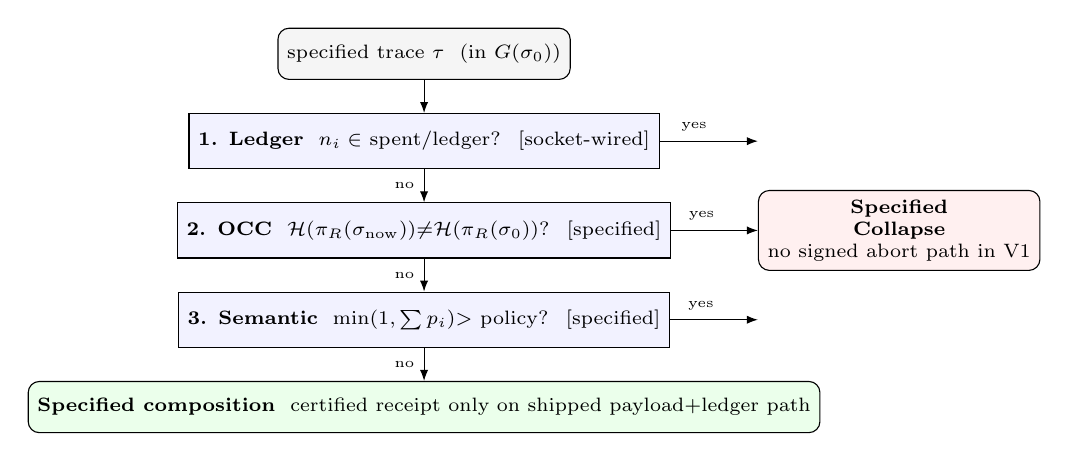
\begin{tikzpicture}[
  node distance=4.2mm,
  box/.style={draw, rounded corners, align=center, font=\scriptsize,
              minimum width=3.5cm, minimum height=6.5mm},
  gate/.style={draw, align=center, font=\scriptsize, fill=blue!5,
               minimum width=3.5cm, minimum height=7mm},
  ar/.style={-{Latex[length=1.4mm]}},
]
\node[box, fill=gray!8] (trace) {specified trace $\tau$ \ (in $G(\sigma_0)$)};
\node[gate, below=of trace] (g1)
  {\textbf{1. Ledger} \ $n_i \in$ spent/ledger? \ [socket-wired]};
\node[gate, below=of g1] (g2)
  {\textbf{2. OCC} \ $\mathcal{H}(\piR(\sigma_{\mathrm{now}})){\ne}\mathcal{H}(\piR(\sigma_0))$? \ [specified]};
\node[gate, below=of g2] (g3)
  {\textbf{3. Semantic} \ $\min(1,\textstyle\sum p_i){>}$ policy? \ [specified]};
\node[box, below=of g3, fill=green!8] (commit)
  {\textbf{Specified composition} \ certified receipt only on shipped payload+ledger path};
\node[box, right=1.1cm of g2, fill=red!6, minimum width=2.7cm] (abort)
  {\textbf{Specified} \\ \textbf{Collapse} \\ no signed abort path in V1};
\draw[ar] (trace) -- (g1);
\draw[ar] (g1) -- node[left, font=\tiny] {no} (g2);
\draw[ar] (g2) -- node[left, font=\tiny] {no} (g3);
\draw[ar] (g3) -- node[left, font=\tiny] {no} (commit);
\draw[ar] (g1.east) -- node[above, font=\tiny, pos=0.35] {yes} (abort.west |- g1.east);
\draw[ar] (g2.east) -- node[above, font=\tiny, pos=0.35] {yes} (abort.west);
\draw[ar] (g3.east) -- node[above, font=\tiny, pos=0.35] {yes} (abort.west |- g3.east);
\end{tikzpicture}
\caption{Specified three-gate validation architecture. Only the ledger and
payload-byte-binding subset is wired in the DAB socket prototype; OCC and
semantic helpers are not runtime-enforced. DAB V1 signs \texttt{CERTIFIED}
outcomes only, not abort responses.}
\label{fig:pipeline}
\end{figure}

\subsection{Receipts as the unit of evidence}
\label{sec:receipts}

The TypeScript decision-receipt protocol defines canonical JSON envelopes with
an exact, validated key set, content-derived identifiers, and signatures over
canonical bytes. Its Node and Python verifiers are exercised by differential
tests; HMAC is local development only and KMS signing is an intended AWS mode.
The separate DAB V1 socket receipt is narrower: it signs a successful
\texttt{CERTIFIED} payload binding, nonce, timestamp, and policy digest. It
does not sign a target, a rejection reason, or an abort status; replay and
mutation responses are status messages rather than independently verifiable
receipts. A signature proves authorization over its signed fields, not the
payload's semantic truth. \statusimpl{}

\subsection{Custody and the egress boundary}
\label{sec:custody}

A-CC (\S\ref{sec:acc}) motivates a custody-layer design in which tool traffic
would exit through a loopback sidecar, digest raw response bytes, inject a
request nonce, and return a signed envelope. Provenance admission is
meet-based on a lattice, so data cannot launder trust by transiting the
agent's context. A byte-level reconciler compares \emph{decoded} tool bytes
against asserted content (decode-before-compare). This is not an end-to-end
claim about the DAB socket gateway: the shipped V1 path does not bind a target
or compose the provenance/custody policy with its HTTP execution. The sidecar
and its SSRF-class exposures --- DNS rebinding and redirect handling --- remain
specified surfaces, not dissolved risks. \statusspec{}

\subsection{End-to-End Scenario: Stopping Trust Laundering}
\label{sec:e2e}

The following is a \emph{specified design scenario}, not a trace of the
currently wired runtime. Consider an adaptive agentic worm that uses indirect
prompt injection to commandeer an agent, instructing it to forward sensitive
customer records to an attacker-controlled endpoint.

\begin{enumerate}
    \item \textbf{Execution in $G(\sigma_0)$:} The agent parses the poisoned record and decides to call \texttt{HTTP\_POST}. The proposed loopback sidecar would treat the call as a speculative write.
    \item \textbf{Declarative Binding ($\Delta_{\mathrm{DE}}$):} The proposed agent runtime normalizes the action into a deterministic JSON payload.
    \item \textbf{Custody Evaluation:} The payload claims to be a legitimate summary of customer data. The proposed byte-level reconciler detects that the destination URL is \emph{agent-asserted} (hallucinated from the prompt injection) rather than \emph{gateway-recorded} (passed through an authorized retrieval tool).
    \item \textbf{Speculative Collapse:} The transaction would fail custody
    evaluation (\S\ref{sec:custody}): the floor demanded by the
    destination-write policy exceeds agent-asserted provenance, so the A-CC
    attempt dies as an \emph{unsatisfiable floor} --- a deterministic lattice
    check, not a semantic judgment (the semantic gate of \S\ref{sec:frechet}
    is a separate, later check over supplied marginals).
    \item \textbf{Evidence Generation:} The proposed gateway discards the speculative buffer and would not execute the network request. A signed \texttt{COLLAPSE} receipt is a future protocol design requirement, not an artifact emitted by DAB V1.
\end{enumerate}

% ============================================================================
\section{Formal Foundations}
\label{sec:formal}

\subsection{The starvation trap and the read-set projection}
\label{sec:starvation}

The naive OCC gate validates the world:
$\mathcal{H}(\sigma_{\mathrm{now}}) = \mathcal{H}(\sigma_0)$. In any live
environment this is a liveness catastrophe. Let environmental writes
unrelated to the trajectory arrive as a Poisson process with rate $\lambda$,
and let a trajectory speculate for time $d$. The probability that
\emph{global} validation succeeds is $e^{-\lambda d}$: for an agent that
reasons for 30\,s in an environment averaging one background write per
second, the commit probability is $e^{-30} \approx 10^{-13}$ --- perpetual
abort. Worse, the abort-retry loop is self-defeating: retries lengthen
exposure, and exposure breeds conflict. This is the \textbf{starvation
trap}: global-state validation converts safety into a denial of liveness.

The repair is the projection operator $\piR$, which restricts validation to
the trajectory's declared read-set --- the tuples actually consulted while
speculating. Validation becomes
$\mathcal{H}(\piR(\sigma_{\mathrm{now}})) = \mathcal{H}(\piR(\sigma_0))$,
and the abort probability depends only on the write rate \emph{into the
read-set}, $e^{-\lambda_R d}$ with $\lambda_R \ll \lambda$. The cost is
stated, not hidden: $\piR$ detects exactly read--write conflicts on declared
dependencies. Predicate-shaped reads (``all alarms currently firing'') must
materialize their result set into the projection or the gate inherits the
phantom problem~\cite{berenson1995critique}; an unfaithfully narrow $\piR$
weakens conflict detection in proportion to what it omits. Serializability
under $\piR$ is therefore conditional on read-set faithfulness --- a property
of instrumentation, not of the gate (Figure~\ref{fig:starvation}).
\statusspec{}

\begin{figure}[t]
\centering
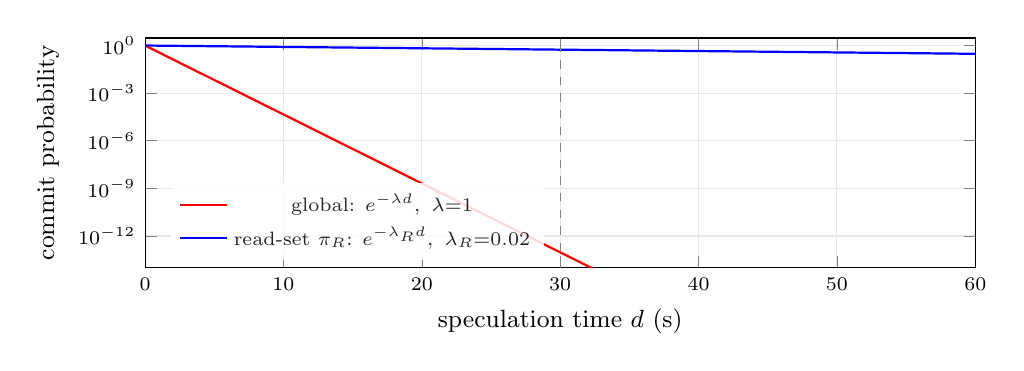
\begin{tikzpicture}
\begin{semilogyaxis}[
  width=\columnwidth, height=4.5cm,
  xlabel={speculation time $d$ (s)}, ylabel={commit probability},
  xmin=0, xmax=60, ymin=1e-14, ymax=3,
  ytick={1,1e-3,1e-6,1e-9,1e-12},
  legend pos=south west,
  legend style={font=\scriptsize, fill=white, fill opacity=0.85, draw=none},
  tick label style={font=\scriptsize}, label style={font=\small},
  grid=both, grid style={gray!18},
]
\addplot[thick, red, domain=0:60, samples=90] {exp(-1.0*x)};
\addlegendentry{global: $e^{-\lambda d},\ \lambda{=}1$}
\addplot[thick, blue, domain=0:60, samples=90] {exp(-0.02*x)};
\addlegendentry{read-set $\pi_R$: $e^{-\lambda_R d},\ \lambda_R{=}0.02$}
\draw[dashed, gray] (axis cs:30,1e-14) -- (axis cs:30,3);
\end{semilogyaxis}
\end{tikzpicture}
\caption{The starvation trap (\S\ref{sec:starvation}). Global-state validation
decays as $e^{-\lambda d}$ --- perpetual abort ($\approx 10^{-13}$ at
$d{=}30$\,s, dashed line, for $\lambda{=}1$ background write/s). Validating only
the read-set projection $\piR$, whose write rate $\lambda_R \ll \lambda$, keeps
the commit probability near $1$. The curves are the analytic Poisson model, not
measurements; read-set faithfulness is the stated cost.}
\label{fig:starvation}
\end{figure}

\subsection{Fr\'echet bounds on cumulative trajectory failure}
\label{sec:frechet}

Per-step screening misses trajectory-level violations: no single action
$a_i$ crosses policy, but the sequence does. Model step $i$'s violation as
an event $F_i$ with marginal $p_i = \mathbb{P}(F_i)$, supplied by upstream
assessors. The deployment-relevant quantity is
$\mathbb{P}(F_{\mathrm{any}}) = \mathbb{P}(\bigcup_i F_i)$ --- and the joint
dependence structure of the $F_i$ is unknown. Assuming independence is not
conservative here; it is the precise mistake our research program exists to
measure, because guardrail failures \emph{correlate}: the same poisoned
context that defeats the step-3 assessment also defeats step 5's. The
Fr\'echet bounds~\cite{nelsen2006copulas,boole1854laws} are the sharp
dependence-free envelope:
\begin{equation}
\max_i\, p_i \;\le\; \mathbb{P}\Big(\bigcup_{i=1}^{k} F_i\Big) \;\le\;
\min\Big(1,\; \sum_{i=1}^{k} p_i\Big),
\label{eq:fh-union}
\end{equation}
with the dual intersection envelope
$\max\!\big(0, \sum_i p_i - (k-1)\big) \le \mathbb{P}(\bigcap_i F_i) \le
\min_i p_i$. The semantic gate implements the upper bound of
\eqref{eq:fh-union} as its trigger: it aborts when
$\min(1, \sum_i p_i)$ exceeds the policy threshold. This is the unique
choice that remains valid under \emph{every} dependence structure, including
the adversarially correlated one (Figure~\ref{fig:frechet}).

\begin{figure}[t]
\centering
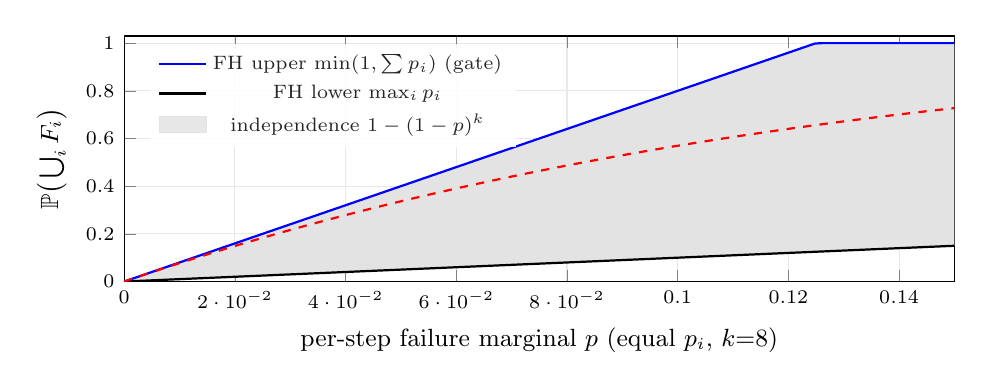
\begin{tikzpicture}
\begin{axis}[
  width=\columnwidth, height=4.7cm,
  xlabel={per-step failure marginal $p$ (equal $p_i$, $k{=}8$)},
  ylabel={$\mathbb{P}\big(\bigcup_i F_i\big)$},
  xmin=0, xmax=0.15, ymin=0, ymax=1.03,
  legend pos=north west,
  legend style={font=\scriptsize, fill=white, fill opacity=0.85, draw=none},
  tick label style={font=\scriptsize}, label style={font=\small},
  grid=both, grid style={gray!18},
]
\addplot[name path=fhupper, thick, blue, domain=0:0.15, samples=120]
  {min(1, 8*x)};
\addlegendentry{FH upper $\min(1,\sum p_i)$ (gate)}
\addplot[name path=fhlower, thick, black, domain=0:0.15, samples=120] {x};
\addlegendentry{FH lower $\max_i p_i$}
\addplot[gray!22] fill between[of=fhupper and fhlower];
\addplot[thick, red, dashed, domain=0:0.15, samples=120] {1-(1-x)^8};
\addlegendentry{independence $1-(1-p)^k$}
\end{axis}
\end{tikzpicture}
\caption{The dependence-free Fr\'echet envelope for union failure over $k{=}8$
steps, equal marginals (\S\ref{sec:frechet}). The semantic gate triggers on the
upper bound, which holds under \emph{every} dependence structure. An
independence assumption (dashed) lies strictly inside the envelope: it would
clear trajectories the worst case flags, under-reporting risk precisely where
correlated guardrail failure lives. Analytic bounds, not measurements.}
\label{fig:frechet}
\end{figure}

Two consequences are worth stating plainly. First, the bound is
conservative by construction, and it saturates: as $k$ grows,
$\sum_i p_i \to 1$ even for well-behaved marginals, and the gate tends
fail-closed --- the starvation trade of \S\ref{sec:starvation} reappearing at
the semantic layer. Long-horizon deployments must either scale the policy
threshold with $k$ or invest in calibrated marginals; the gate makes that
trade explicit rather than hiding it in an independence assumption. Second,
the gate's output is only as meaningful as its inputs: it computes a bound
over supplied marginals and does not manufacture information about content.
Equation~\eqref{eq:fh-union}'s helper (\texttt{evaluateSemanticGate})
is unit-tested against hand-computed bounds. \statusunit{}

\subsection{Model checking with mutants, and the bug it caught}
\label{sec:tla}

Six TLA+ baselines cover the enforcement design: the provenance lattice's
admission monotonicity, the speculative collapse state machine, the transport
boundary (where the byte reconciler is shown to be load-bearing rather than a
parser accident), tenant isolation, the nonce ledger, and the execution
boundary. Model checking that can only pass is theater, so every baseline with
a seeded counterexample is paired with a \emph{mutant} model; the harness
requires baselines to verify clean and mutants to reproduce their violations.
Five of the six baselines have mutants; raw TLC logs are committed artifacts.

The discipline caught us. The original nonce-ledger baseline violated its own \texttt{NoReplays} invariant due to a subtle interaction between garbage collection (GC) and state expiration. TLC produced the following counterexample trace:

\begin{enumerate}
    \item \textbf{Speculate:} Agent submits transaction with \texttt{nonce = X}.
    \item \textbf{Commit:} Gateway admits \texttt{X}, adding it to $\mathcal{L}_{\mathrm{nonce}}$.
    \item \textbf{GC Tick:} \texttt{TTL} expires. \texttt{GarbageCollect} removes \texttt{X} from $\mathcal{L}_{\mathrm{nonce}}$ to bound memory.
    \item \textbf{Replay:} Attacker replays the original transaction. Because \texttt{X} is no longer in $\mathcal{L}_{\mathrm{nonce}}$, the gateway treats it as a fresh request and admits it again.
\end{enumerate}

The flaw was a true positive in the shipped design, not an artifact of the model. The repair introduced the spent-tombstone set ($S_{\mathrm{spent}}$): GC now \emph{archives} rather than \emph{forgets}. Admission requires $n_i \notin \mathcal{L}_{\mathrm{nonce}} \wedge n_i \notin S_{\mathrm{spent}}$. We propagated this fix spec-first into the Rust implementation. The gateway initially retained TTL-eviction semantics --- diverging from the verified model by exactly the refuted behavior --- and was then brought into conformance: \texttt{cleanup\_expired()} archives into a spent set, and a nonce consumed at $T$ is rejected at $T+3601$. One bounded caveat survives and is stated in \S\ref{sec:nonclaims}: the in-process tombstone set is capacity-bounded, and pruning at capacity reopens a theoretical replay window for sufficiently old nonces.

\textbf{Refinement mapping conjecture.} We define the state abstraction function $\alpha: S_{\mathrm{runtime}} \to S_{\mathrm{spec}}$ mapping runtime gateway memory state $S_{\mathrm{runtime}}$ to abstract TLA+ variables $S_{\mathrm{spec}}$. The refinement simulation conjecture states that for every implementation step $S \xrightarrow{\tau} S'$, the abstract state either stutters or executes a valid specification transition:
\begin{equation}
\alpha(S) = \alpha(S') \;\lor\; \alpha(S) \xrightarrow{\tau_{\mathrm{spec}}} \alpha(S').
\label{eq:refinement-sim}
\end{equation}

% ============================================================================
\section{Evaluation}
\label{sec:eval}

\noindent\textbf{Setup disclosure.} Measurements in this section come from
recorded runs at repository HEAD on a single host: Apple M1 (8\,GB RAM),
macOS (Darwin 24.5.0, arm64), Node v22.22.3, single process, no network, no
KMS. TLC runs use tla2tools \tlatoolversion{}; raw reference logs are
committed under \path{proofs/tla/artifacts/} and \path{proofs/dab/artifacts/},
while \path{artifacts/proofs/} contains generated summaries. Nothing here is
a cloud measurement, and no live-AWS evidence is
claimed. Every number maps to a re-runnable command in the artifact
(\S\ref{sec:artifact}). One host is one host: no cross-machine claim is
available here, and reported dispersion describes this machine's scheduling
noise only.

\subsection{Superseded evidence}
\label{sec:superseded}

An earlier revision of this paper drew its headline detection and latency
numbers from \texttt{dab/bench/}. We retract those numbers and record why,
because the failure is instructive and because a correction a reader cannot
locate is not a correction.

Several suites in that directory reported \texttt{detected: true} while
invoking no component of the system under test. A nonce-swap check built two
requests with differing payloads and a shared nonce, then asserted that the
payloads differed and the nonces matched --- both true by construction, with
no ledger, gateway, or verifier consulted. A replay check consulted a
\texttt{Set} declared in the benchmark file, measuring that
\texttt{Set.prototype.has} works, while the Rust tombstone ledger it was
cited as exercising was never called. Unicode checks asserted properties of
\texttt{String.prototype.normalize}. The mutation suite computed real digests
over real inputs but thereby demonstrated SHA-256's avalanche property --- a
property of SHA-256, expected of any correct hash. The directory imports only
\texttt{node:crypto} and \texttt{node:perf\_hooks}. It is now quarantined,
with a README stating it is not evidence about this system.

That quarantine was, until 2026-08-11, enforced one indirection too high, and
we record the gap rather than quietly closing it. The guard asserted that no
\emph{workflow file} names the directory. That held --- the artifact workflow
says \texttt{make reproduce} --- while the chain beneath it
(\texttt{reproduce.sh} $\to$ \texttt{run-attacks.sh}) ran the quarantined bench
and let its exit status gate the reproduction, printing ``all adversarial
evidence green'' over the result. An earlier revision of this subsection cited
that guard as ``a test asserting no workflow treats it as such'', which was true
of the file text and false in effect. The bench now runs non-gating under a
\texttt{quarantined\_smoke} key, and the guard follows the call graph rather than
the spelling of the call site. The general form is worth stating: \emph{a
containment check that matches on the name of a caller does not contain
anything a caller can reach}.

The consequent retractions are tracked as R1--R5 and R10 in the repository's
retraction ledger (\texttt{docs/research/EXPERIMENTS.md}):

\begin{itemize}
\item \textbf{Detection rates from that corpus} are withdrawn. Superseded by
  \S\ref{sec:eval-corpus}, which runs the malicious corpus through the real
  standalone verifier, stratifies by which check rejected, and carries a
  control arm.
\item \textbf{``Unicode spoofing is entirely eradicated at the TCB
  boundary''} is withdrawn --- an absolute-security claim whose evidence was
  a TypeScript compile error in a benchmark that never ran. Measurement since
  shows the canonicalizer \emph{over}-discriminates NFC/NFD, and that Unicode
  handling diverges across runtimes.
\item \textbf{A Wilson interval computed at $n=2$} and presented as a robust
  statistical lower bound is withdrawn; at $2/2$ that bound falls below
  $0.4$. Intervals are no longer computed below $n=30$, nor over a census.
\item \textbf{The latency figures and the $1{,}333\%$ relative overhead} are
  withdrawn: that harness reported no dispersion and used a $0.5\,\mu$s no-op
  denominator. Superseded by \S\ref{sec:eval-perf} --- p50 with IQR against a
  parse-only baseline. The accompanying throughput figure has \emph{no}
  replacement and is withdrawn outright; the superseding experiment does not
  measure throughput, and we do not substitute a number we did not take.
\end{itemize}

The general rule this cost us: a detection benchmark is evidence only if
breaking the mechanism it depends on stops the detection. That discriminator
is now applied to the corpus of \S\ref{sec:eval-corpus}, and is why its
result is reported at all.

\subsection{Model checking}
\label{sec:eval-tla}

\begin{table}[t]
\centering\scriptsize
\begin{tabularx}{\columnwidth}{@{}Yr>{\raggedright\arraybackslash}p{2.25cm}@{}}
\toprule
\textbf{Model} & \textbf{Distinct states} & \textbf{Result}\\
\midrule
ProvenanceLattice          & \plstates{}    & clean \\
\quad\emph{mutant}         & \mutrange{}    & violation reproduced \\
SpeculativeCollapse        & \scstates{}    & clean \\
\quad\emph{mutant}         & \mutrange{}    & violation reproduced \\
TransportBoundary          & \tbstates{}    & clean \\
\quad\emph{mutant}         & \mutrange{}    & violation reproduced \\
TenantIsolation            & \tistates{}    & clean \\
\quad\emph{mutant}         & \mutrange{}    & violation reproduced \\
DAB\_NonceLedger           & \nlstates{}    & clean (incl.\ temporal) \\
\quad\emph{mutant}         & \mutrange{}    & \texttt{NoReplays} violated \\
DAB\_ExecutionBoundary     & \ebstates{}    & clean --- \emph{no mutant} \\
\bottomrule
\end{tabularx}
\caption{TLC results in the recorded evidence snapshot (tla2tools
\tlatoolversion{}; raw logs committed).
\textbf{Baseline counts are exact and reproducible}; they exhaust the bounded
state space, and the five that predate the 2026-08 toolchain change re-derived
byte-identically across it (\texttt{TenantIsolation}, checked 2026-08-12, has
run only under the current pin; its count matches the expectation pre-registered
in \texttt{proofs/tla/README.md} before the run).
\textbf{Mutant counts are ranges, and deliberately so} (retraction R11): a mutant
halts at the first counterexample under \texttt{-workers auto}, so the count
depends on thread scheduling rather than on the model. Ranges are $n=10$ per
mutant on one host at one commit. The \emph{verdict} is what reproduces; the
count is not, and was previously reported as a constant.
Baselines must verify clean; mutants must reproduce their seeded violations.
Six baselines, \emph{five} mutants: \texttt{DAB\_ExecutionBoundary} has no
seeded mutant, so its clean result is one-sided. These are bounded models of
the design, not proofs of the implementation.}
\label{tab:tlc}
\end{table}

Table~\ref{tab:tlc} summarizes six baselines and five mutants. The
two-sided oracle matters: a harness that can only report success cannot
distinguish a verified invariant from a vacuous one. The mutant rows are the
evidence that the invariants have teeth; the \texttt{NoReplays} mutant in
particular reproduces the historical design flaw of \S\ref{sec:tla} as a
permanent regression witness. \texttt{TenantIsolation} is the newest pair
(2026-08-12) and a lesson in what this table is for: its first version was
tautological --- the invariant restated the guard of the only action that could
produce an allow entry, so no behaviour could violate it --- and unbounded, so
TLC could not terminate. The rebuilt model makes ownership mutable and routes
grant decisions through a cache that transfer must invalidate; the mutant
deletes exactly that invalidation and violates through a stale-cache grant.

By that same standard we must mark our own gap: \texttt{DAB\_ExecutionBoundary}
is checked clean over \ebstates{} distinct states but ships \emph{no} mutant, so
nothing demonstrates its invariants can fail. Its row is exactly the one-sided
result the rest of this table exists to rule out, and we count it as unverified
teeth rather than as a sixth mutant.

\subsection{Adversarial corpus}
\label{sec:eval-corpus}

At HEAD, the malicious-fixture corpus is run through the \emph{real}
standalone verifier (\texttt{verifiers/node/ghost\_receipt\_verify.mjs}) with
options sourced from the reproducibility manifest, and every detection is
stratified by \emph{which} check rejected. \evthreeintrinsic{} mutations are
rejected by verifier rules alone; \evthreeaggregate{} detectable mutations are
rejected somewhere in the pipeline; \evthreeundetected{} go undetected. A
further \evthreeboundary{} fixtures are ones the corpus \emph{declares should
be accepted} --- documented boundaries, excluded from the rate rather than
silently counted as successes. The control arm --- the unmutated base
fixtures --- passes \evthreecontrol{}. That arm is what makes the number mean
anything: a verifier that rejected every input would also score 100\%
detection.

We quote the stratified figure rather than the aggregate. Of the rejections,
one is a JSON load failure on malformed input, which no verifier \emph{rule}
can take credit for, and two come only from a declared consumer expectation.
That last stratum is the thesis in miniature: a byte-identical,
cryptographically valid receipt issued to tenant A and presented to a tenant-B
consumer. No verifier rule can reject it --- the receipt is \emph{correct}.
Only the consumer's declared expectation distinguishes it, which is precisely
$\mathrm{Sound}(C,\Sigma,P)$ depending on $P$ with $C$ unchanged.

Provenance is \textbf{census}, not sample: these are exact counts over a
hand-authored corpus whose size is an authoring decision, so no confidence
interval is attached. A curated corpus has no sampling variability to
describe (\S\ref{sec:superseded} records this paper's own earlier violation
of that rule).

Crucially, these detections are \emph{load-bearing}. A metamorphic guard
forces each verifier check to pass in turn and confirms the dependent
detections then stop: \evfourloadbearing{} checks are load-bearing for named
fixtures, and with \emph{every} check forced to pass, the only surviving
rejection is a parse failure. A check that still reports success once its
mechanism is broken measures nothing --- and this discriminator exists
because an earlier corpus in this project failed it
(\S\ref{sec:superseded}). Two checks are not isolable by any fixture by
construction, and one has no dependent fixture at all; we report that as a
\emph{corpus} gap rather than a useless check.

\paragraph{Coverage boundary.} The corpus contains \emph{no} fixtures for: a
compromised signer able to produce valid signatures over mutated payloads,
multi-field coordinated mutations, chain- or checkpoint-level attacks across
many receipts, ledger completeness or omission attacks, timing and
side-channel attacks, key-rotation-boundary attacks, or any live AWS/KMS
custody attack. A \evthreeintrinsic{} result says nothing about these, and it
is not a statement about unmodeled attackers, the Rust TCB under deployment
conditions, or semantic-layer deception.

\paragraph{A model-internal calculation, reported as such.}
Separately from the measurements above, \texttt{dab/bench/formal\_games.ts}
computes an attacker advantage of \globaladvantage{} across four security
games at \benchtrials{} trials each (mutation resistance, replay resistance,
cross-transaction binding, serialization ambiguity). We report this as what
it is: a calculation over the file's own declared attacker model, invoking no
Ghost-Ark component. It is not evidence about the implementation, and we do
not count it among the results above. Under a rule-of-three
reading~\cite{hanley1983rule} a zero rate over $10^4$ trials bounds the true
per-trial win probability below $\approx 3\times10^{-4}$ \emph{within that
model} --- which says nothing about the deployed system, and nothing about
attacks outside the modeled family.

On indirect prompt injection: the published InjecAgent
benchmark~\cite{zhan2024injecagent} reports attack success rates up to 47\%
for a ReAct-prompted GPT-4 agent in its enhanced setting. Under \ghostark{}'s
custody model the corresponding trust-laundering move is \emph{structurally}
unsatisfiable --- injected in-context text carries no gateway envelope, so it
cannot meet floors above agent-asserted provenance, and our in-repository
scenario tests confirm the admission rule blocks the modeled laundering
pattern. We deliberately do not report this as ``ASR reduced from 47\% to
0\%'': we have not re-run the InjecAgent dataset against a live model behind
\ghostark{}, and the published 47\% baseline was measured under different
conditions. The honest statement is architectural non-satisfiability under
the modeled floor semantics, evidenced by unit and scenario tests.
% NOTE: a live InjecAgent replication behind the gateway is future work
% (docs/defense/DEFENSE_ANCHOR.md); do not upgrade the claim before then.

\subsection{Performance}
\label{sec:eval-perf}

\begin{table}[t]
\centering\scriptsize
\begin{tabular}{@{}lrrr@{}}
\toprule
\textbf{Path} & \textbf{p50} & \textbf{IQR} & \textbf{$\times$base}\\
\midrule
parse only          & \evtwobasepfifty{}   & \evtwobaseiqr{}    & ---\\
canonicalize        & \evtwocanonpfifty{}  & \evtwocanoniqr{}   & \evtwocanonratio{}$\times$\\
canon. + digest     & \evtwodigestpfifty{} & \evtwodigestiqr{}  & \evtwodigestratio{}$\times$\\
HMAC verify         & \evtwohmaconlypfifty{} & \evtwohmaconlyiqr{} & \evtwohmaconlyratio{}$\times$\\
full HMAC           & \evtwohmacpfifty{}   & \evtwohmaciqr{}    & \evtwohmacratio{}$\times$\\
full RSA-PSS        & \textbf{\evtworsapfifty{}} & \evtworsaiqr{} & \textbf{\evtworsaratio{}$\times$}\\
\bottomrule
\end{tabular}
\caption{Receipt verification cost in \emph{microseconds}, p50 with IQR.
\evtwoiters{} measured iterations after 500 discarded warmup iterations;
canonical payload 1552 bytes; host \evtwohost{}. Every result feeds an $O(1)$
sink so the JIT cannot eliminate the work. Paths are parse-only,
canonicalize-only, canonicalize-and-digest, HMAC verification, full HMAC, and
full RSA-PSS; the baseline is parse-only.}
\label{tab:perf}
\end{table}

Table~\ref{tab:perf} reports verification cost with a baseline, as p50 with
IQR --- a bare p50 is not a result. Asymmetric verification dominates: the
full RSA-PSS path is $\approx$5.4$\times$ the full HMAC path and
\evtworsaratio{}$\times$ the parse baseline. Canonicalization is
\emph{not} the bottleneck, at \evtwocanonratio{}$\times$ baseline --- an order
of magnitude below the asymmetric signature. The harness also declares subset
orderings (a superset arm cannot be cheaper than its subset) and audits them;
all four hold at \evtwoiters{} iterations. At $n=2000$ an inversion appeared
intermittently between two arms $\approx$1\,$\mu$s apart with IQRs of
$2+\,\mu$s, unresolvable at that sample size; the harness reported the
inversion rather than publishing an impossible number, and the default was
raised.

The choice of denominator is the point. A relative-overhead figure is only
as meaningful as its baseline: measured against a no-op dispatch, any real
work looks catastrophic, and a four-digit percentage carries no decision
content. \texttt{json-parse-only} is chosen instead because it is what a
consumer unavoidably pays to read the document at all, which makes
\evtworsaratio{}$\times$ an actionable ratio rather than a rhetorical one.
An earlier version of this paper headlined a $1{,}333\%$ overhead against a
$0.5\,\mu$s no-op baseline, drawn from a harness with no dispersion reporting
and no baseline discipline; that figure and its source are retracted in
\S\ref{sec:superseded}.

\paragraph{Coverage boundary.} Single host, single process, no concurrency,
no adversarial input sizing, and no AWS or KMS network path. The IQR
describes \emph{this machine's} scheduling noise, not variation across
machines --- we have not measured a second host, so no cross-machine claim is
available. These are not throughput numbers and not a performance guarantee.
Signing latency under KMS and all network costs are excluded and will
dominate in the intended cloud mode (\S\ref{sec:nonclaims}). ``Fast'' is not
a property we claim; ``microseconds of in-process verification on one named
host, unmeasured I/O excluded'' is.

\textbf{Concurrent TCB throughput, measured.} Table~\ref{tab:perf} times
\emph{TypeScript} receipt verification, single-threaded on one host; it
reports latency, not throughput, and is not a load test. We therefore also
measure the
Rust TCB directly under concurrency. A prior throughput run was taken against a
lock-free replay-admission implementation. The current implementation instead
serializes the short active-to-spent nonce transition so its check-and-commit
semantics match the replay invariant; the prior throughput figures are therefore
not carried forward as a claim about the current code. The harness remains
two-sided: every in-capacity operation must admit and every at-capacity operation
must refuse, or the run exits non-zero. A current throughput result requires a
fresh recorded run and still excludes Unix-socket transport and all network I/O;
it would not be a deployed-load claim (\S\ref{sec:nonclaims}).

\subsection{A disclosed harness bug}
\label{sec:eval-bug}

An earlier revision of this benchmark scored two suites backwards: the
replay game counted a \emph{detected} replay as an attacker win (reporting
advantage $\approx 0.998$ where correct accounting yields 0), and one
mutation probe inverted its detection predicate, yielding an aggregate
``advantage'' of $\approx 0.25$ that contradicted the design's own ledger
semantics. The error was in the harness's accounting, not the enforcement
path --- but for a period the repository's own artifact report published the
red result rather than patching around it, and the fix landed as an ordinary
reviewed commit. We disclose this for the same reason we ship mutant models:
an evaluation pipeline that cannot be caught being wrong cannot be trusted
when it says it is right.

That harness has since been retired from the evidence base entirely, for a
deeper defect than mis-scoring: several of its suites reported detection
without invoking any component under test (\S\ref{sec:superseded}). Correct
accounting over a tautological check still measures nothing.

\subsection{The replay window, measured}
\label{sec:replaywindow}

The ledger gate's one honest weakness (\S\ref{sec:nonclaims}, item 6) is that
its in-process tombstone set is capacity-bounded: at capacity, pruning
reopens a replay window for old nonces. Most papers state such a caveat and
stop. We measure it. Driving the real \texttt{ReplayLedger} at capacity $C$
after creating $K$ tombstones (TTL$=0$ for a deterministic boundary) and
counting how many consumed nonces become replayable (\texttt{!exists}, exactly
the condition under which \texttt{consume} would re-accept) yields, across
capacities from $8$ to $100$ and $K$ up to $1000$ (recorded in
\texttt{RECORDED\_REPLAY\_WINDOW.txt}), an exact law:
\begin{equation}
\text{replay window} \;=\; \max\!\big(0,\; K - C\big).
\label{eq:window}
\end{equation}
Figure~\ref{fig:window} shows the knee at $K{=}C$: below capacity the window
is empty (every tombstone is retained), above it the window grows one-for-one.
The measurement also surfaces a \emph{second} finding the caveat alone hides:
because the in-process set is a \texttt{HashSet}, the pruned membership is
implementation-arbitrary, not age-ordered --- so a durable production store
must use time-ordered eviction, not merely more capacity. The bound is now a
number an operator can size against, not a hand-wave: with the default
$C{=}500{,}000$ the window stays empty until more than half a million distinct
nonces outlive their TTL between compactions.

\begin{figure}[t]
\centering
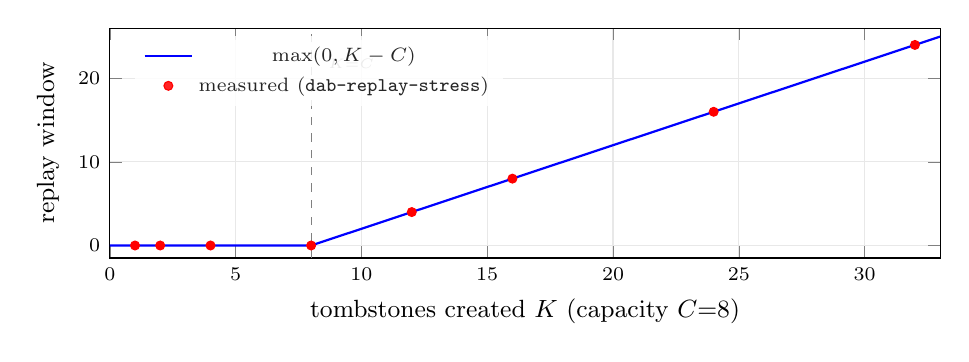
\begin{tikzpicture}
\begin{axis}[
  width=\columnwidth, height=4.5cm,
  xlabel={tombstones created $K$ (capacity $C{=}8$)},
  ylabel={replay window},
  xmin=0, xmax=33, ymin=-1.5, ymax=26,
  legend pos=north west,
  legend style={font=\scriptsize, fill=white, fill opacity=0.85, draw=none},
  tick label style={font=\scriptsize}, label style={font=\small},
  grid=both, grid style={gray!18},
]
\addplot[thick, blue, domain=0:33, samples=100] {max(0, x-8)};
\addlegendentry{$\max(0, K-C)$}
\addplot[only marks, mark=*, mark size=1.6pt, red] coordinates {
  (1,0) (2,0) (4,0) (8,0) (12,4) (16,8) (24,16) (32,24)
};
\addlegendentry{measured (\texttt{dab-replay-stress})}
\draw[dashed, gray] (axis cs:8,-1.5) -- (axis cs:8,26);
\node[font=\tiny, gray, anchor=south west] at (axis cs:8.3,20) {$K{=}C$};
\end{axis}
\end{tikzpicture}
\caption{The bounded replay window, measured (\S\ref{sec:replaywindow}). Below
capacity the window is empty; above it, every additional tombstone is one more
replayable nonce. Measured points fall exactly on
$\max(0,K-C)$~\eqref{eq:window}. This is a measurement of the mechanism's own
stated limitation, not of its strength.}
\label{fig:window}
\end{figure}

\subsection{Deployment Sketch: \ghostark{} on AWS}
\label{sec:deployment}

This subsection is a \emph{design target}, not an evaluated system: no
live-cloud measurement appears in this paper, and items 3 and 7 of
\S\ref{sec:nonclaims} govern everything below. With that boundary stated,
the architecture maps onto standard cloud infrastructure as follows. The
untrusted agent runtime (e.g., a ReAct loop calling a hosted model API)
would run in an isolated container, with the \ghostark{} gateway as an
out-of-process sidecar; the speculative buffer $G(\sigma_0)$ stays local to
the gateway. At commit time the ledger gate's tombstone set would move from
the in-process bounded structure to a durable KV store using conditional
writes (the posture already recommended for the capacity caveat of
\S\ref{sec:nonclaims}, item 6), and the OCC gate --- still \statusspec{} ---
would validate $\piR$ digests against the same store. Receipt signing in the
intended cloud mode uses KMS asymmetric keys referenced by immutable key
ARNs, per the repository's signing boundary. Cloud I/O (network round-trips,
KMS calls) would dominate the microsecond-scale in-process
verification of \S\ref{sec:eval-perf} by orders of magnitude; the validation
\emph{structure} --- the same three-gate conjunction, the same receipt
semantics --- is what carries over, while cloud-mode latency, availability,
and failure behavior remain unmeasured claims we do not make.

% ============================================================================
\section{Limitations and Non-Claims}
\label{sec:nonclaims}

\ghostark{} verifies what was \emph{recorded, signed, policy-bounded, and
replayable under its verifier rules}. Each item below is a boundary we
consider part of the contribution, not an escape hatch.

\begin{enumerate}
\item \textbf{No semantic safety.} Nothing here certifies that agent output
is true, aligned, or safe. The semantic gate bounds a function of supplied
marginals; garbage marginals yield a well-computed bound over garbage.
\item \textbf{Bounded models, not verified implementations.} TLC results are
exhaustive only within stated bounds and hold for the models; conformance of
the Rust/TypeScript implementations is tested, not proved.
\item \textbf{OCC gate unimplemented at runtime.} $\piR$ validation exists as
specification and tested receipt schema; no runtime enforces it yet.
Serializability claims are therefore design-level, and conditional on
read-set faithfulness even then.
\item \textbf{DAB V1 signs certified executions only.} The socket prototype
signs \texttt{CERTIFIED} receipts whose payload binding is independently
verified. It does not sign a request target, rejection reason, or abort
status; replay and mutation responses are unsigned, and malformed or
execution-failure paths may emit no receipt. The independent verifier accepts
\texttt{CERTIFIED} receipts only. Thus this paper makes no claim that every
abort or decision has a signed, independently replayable receipt.
\item \textbf{Modeled attacker only.} The corpus result
(\S\ref{sec:eval-corpus}) is a census over hand-authored mutation, replay,
encoding, and cross-tenant fixtures run against the verifier; its coverage
boundary is stated there. No claim covers unmodeled attacks, the deployed
TCB, or availability. The four-game \globaladvantage{}-advantage figure is a
model-internal calculation, not a measurement of this system.
\item \textbf{Bounded tombstone capacity.} The in-process spent set prunes
at 500{,}000 entries (env-tunable); a nonce older than both TTL and tombstone
capacity has a replay window --- \emph{measured} to be exactly $\max(0,K-C)$
for $K$ tombstones at capacity $C$, with implementation-arbitrary membership
(\S\ref{sec:replaywindow}, Figure~\ref{fig:window}). Durable external stores
with time-ordered eviction (e.g., conditional writes against a database) are
the intended production posture and are not implemented here.
\item \textbf{No live-cloud evidence.} KMS-mode signing, Bedrock-path
integration, and all AWS-live behavior are design targets; no live-AWS
measurement appears in this paper.
\item \textbf{No attestation.} Signing proves authorization over payload
bytes; it does not prove runtime integrity, and no enclave/PCR-bound flow is
claimed.
\item \textbf{Confused deputy within clearance} (\S\ref{sec:oos}) is
mitigated by routing policy at best; the lattice checks floors, not intent.
\item \textbf{Single node.} All ledgers are single-writer; multi-node
consensus over ledger state is future work, not a property of this system.
\item \textbf{No detector efficacy claims.} Where upstream assessors supply
$p_i$, their hit rates are theirs; this paper certifies none of them.
\end{enumerate}

% ============================================================================
\section{Related Work}
\label{sec:related}

\textbf{Transactions and isolation.} The validation-phase structure is
Kung--Robinson OCC~\cite{kung1981occ}; the speculative-buffer discipline
descends from STM~\cite{shavit1995stm,herlihy1993tm}; serializability theory
and the anomaly vocabulary are classical~\cite{papadimitriou1979serial,
berenson1995critique,bernstein1981concurrency}. \ghostark{}'s difference is
the transaction participant: a stochastic planner whose failure modes are
adversarial and correlated, not merely concurrent.

\textbf{Information flow.} The provenance lattice is in the Denning
lineage~\cite{denning1976lattice} with language-based descendants such as
JIF~\cite{myers1997jflow}; the custody twist is that labels are
\emph{cryptographically evidenced} classes (gateway-recorded vs.\
agent-asserted) rather than compiler-tracked types.

\textbf{Agent security.} Indirect prompt injection is systematized
in~\cite{greshake2023not}; InjecAgent~\cite{zhan2024injecagent} benchmarks
it for tool-integrated agents; ReAct~\cite{yao2023react} is the canonical
coupled loop this paper's Table~\ref{tab:isolation} places at read
uncommitted. Sandbox isolation is complementary at two layers ---
infrastructure microVMs (Firecracker~\cite{agache2020firecracker}) and
agent-focused confinement stacks such as NVIDIA NemoClaw, which runs the
agent under Landlock/seccomp/network-namespace isolation with policy-gated
egress~\cite{nemoclaw2026}. Both bound the blast radius of a \emph{process};
\ghostark{} specifies a validation phase and can evidence certified outcomes
from its current socket subset --- Table~\ref{tab:isolation}'s
read-committed row is exactly the sandbox posture, strengthened in the
specified design with validation.

\textbf{Transparency.} Receipt chains and independent replay are in the
spirit of Certificate Transparency~\cite{laurie2014ct}: shrink the trusted
statement from ``the system behaved'' to ``the log is append-only and the
artifacts verify''.

\textbf{Formal methods in systems.} The TLA+/TLC
workflow~\cite{lamport2002specifying,yu1999model} and its industrial use at
scale~\cite{newcombe2015amazon} inform the harness; the mutant-oracle
discipline is mutation testing~\cite{demillo1978mutation} applied to
specifications rather than code.

% ============================================================================
\section{Artifact Availability}
\label{sec:artifact}

The repository ships a reviewer container (Ubuntu 22.04, Node v22.22.3,
Rust 1.97.1, a JDK, pinned tla2tools, and TeX Live) and a paper-specific,
fail-closed evidence gate. \texttt{make paper-evidence} runs E2, E3, E4,
TLC, the full test suite, and a tracked-source claim scan; its exit status is
the result. It does \emph{not} invoke \path{dab/bench/}, which remains
quarantined. The older \texttt{make reproduce} is a broader artifact workflow
and is not the reproduction command for this manuscript's headline evidence.

The manifest \path{docs/paper/evidence-snapshot.v1.json} is the source for
the manuscript macros, \texttt{README-AE.md}, toolchain versions, evidence
paths, and recorded counts. Its release check requires these generated
surfaces to remain byte-synchronous. Test counts are a lower-bound snapshot:
a reproduction is successful when the suite is green and is not below
\testcount{} tests in \testfiles{} files, not when it matches a fixed total.
The claim scan likewise applies to the tracked source revision
(\claimfiles{} scannable files at the recorded revision, zero violations);
a normal working-tree scan intentionally changes as generated or untracked
files appear.

% ============================================================================
\section{Conclusion}
\label{sec:conclusion}

The agent-security debate keeps asking how to make the model trustworthy.
Databases stopped asking the analogous question about transactions fifty
years ago: assume the client is wrong, isolate its speculation, validate at
commit, and log everything. \ghostark{} is that posture applied to
non-deterministic compute --- a ledger gate that model checking humbled and
then hardened, an OCC discipline honest about its liveness trade, a semantic
bound honest about its inputs, and signed \texttt{CERTIFIED} receipts for the
subset of socket outcomes that the shipped V1 path records.
What it refuses to claim is part of the design: a skeptical reviewer should
be able to distrust the authors, the README, and the model, and still
replay the digest, verify the signature, map each claim to its evidence, and
reproduce the failure boundary.


\ifdoubleblind
% Omitted from the anonymous-review rendering.
\else
\section*{Acknowledgments}
The author utilized an AI assistant to help format, refine, and draft the prose
of this manuscript; however, the architectural design, formal modeling,
experimental execution, and final conclusions are the sole work of the author,
who takes full responsibility for the contents of this paper.
\fi
% ============================================================================
\appendix
\section{Artifact Appendix}
\label{sec:appendix}

\subsection{Abstract}
The artifact is the complete repository: the TypeScript enforcement runtime
and receipt schema, the Rust gateway sources, six TLA+ baselines with five
seeded mutants and their recorded TLC logs, the malicious-fixture corpus and its
metamorphic guard, the verification-cost harness, the claim-language scanner
that gates the repository's own documentation (including this manuscript's
\texttt{.tex} source), and a paper-evidence pipeline that fails closed on
E2/E3/E4, TLC, tests, and the tracked-source scan. It is the reproduction
path for the evidence cited in Tables~\ref{tab:tlc}--\ref{tab:perf}.

\subsection{Checklist}
\begin{itemize}
\item \textbf{Program:} Node.js v22.22.3 (TypeScript via native
  type-stripping), Rust 1.97.1 for the DAB crates, and JDK $\ge$ 11 for TLC
  (pinned \texttt{tla2tools.jar} \tlatoolversion{}).
\item \textbf{Run-time environment:} Linux x86\_64 or macOS arm64; or the
  provided Ubuntu 22.04 reviewer container (zero host setup beyond Docker).
\item \textbf{Hardware:} any commodity machine. The paper's latency numbers
  are from an Apple M1 (8\,GB). We have not measured a second host, so we
  claim no cross-machine reproduction: expect the \emph{ordering} of arms and
  the baseline ratios to hold, and absolute microseconds not to.
\item \textbf{Metrics:} stratified detection counts with a control arm, TLC
  distinct-state counts, verification-cost p50 with IQR, test counts,
  claim-gate status.
\item \textbf{Expected wall-clock:} host- and cache-dependent. The
  \texttt{make paper-evidence} report records the duration of each gate; no
  fixed wall-clock claim is part of the evidence snapshot.
\item \textbf{Public availability:} the repository is public; an immutable
  archived snapshot (e.g., Zenodo DOI) is the intended citable artifact.
\end{itemize}

\subsection{Claims mapped to commands}
The authoritative map is \texttt{README-AE.md} at the repository root; the
digest:
\begin{itemize}[leftmargin=*, itemsep=1pt]
\raggedright
\item Table~\ref{tab:tlc} (six models clean, five mutants violate, baseline
  state counts): \texttt{bash scripts/run-proofs.sh} $\rightarrow$ generated
  \path{artifacts/proofs/proofs_summary.json}; committed raw reference logs
  are under \path{proofs/tla/artifacts/} and \path{proofs/dab/artifacts/}.
\item Corpus detection (\evthreeintrinsic{} verifier-intrinsic,
  \evthreecontrol{} control arm, \evthreeundetected{} undetected):
  \texttt{npm run experiment:e3}. Exact counts --- census provenance.
\item That those detections are load-bearing rather than tautological:
  \texttt{npm run experiment:e4}.
\item Table~\ref{tab:perf}: \texttt{npm run experiment:e2}. The arm ordering
  and baseline ratios reproduce; absolute microsecond values are
  machine-dependent, and the IQR is this host's scheduling noise.
\item Test snapshot (\testcount{}/\testfiles{}): \texttt{npm test}. A green
  suite must not fall below the snapshot; it may legitimately grow.
\item Claim gate (\claimfiles{} tracked source files, 0 violations):
  run \texttt{node tools/research/check-forbidden-claims.mjs} with
  \texttt{--tracked}. The
  normal working-tree scan is deliberately not compared with this count.
\item Semantic-gate bound (\S\ref{sec:frechet}):
  the focused \texttt{semanticAuditReceipt.test.ts} Vitest file.
\item Full paper-evidence roll-up: \texttt{make paper-evidence}. The
  container invocation is listed in \texttt{README-AE.md}; exit code 0 iff
  every paper-evidence stage passed.
\end{itemize}

\subsection{\texorpdfstring{The gateway$\leftrightarrow$verifier round-trip and its enforcement}{Gateway-verifier round-trip and its enforcement}}
The Rust gateway and the independent verifier agree on a real ed25519
signature over a domain-separated canonical message including
\texttt{policy\_digest}. A recorded, reproducible round-trip
(\path{dab/roundtrip/}) shows a gateway-emitted \texttt{CERTIFIED} receipt
verifying, while tamper, mutation, and wrong-key variants are rejected with
specific errors. The local socket E2E
(\path{dab/roundtrip/run_socket_e2e.sh}) drives the running gateway with the
Rust agent client through a workspace-local Unix socket. It verifies a
certified receipt, observes a replay rejection for a reused nonce, and
byte-compares the sink's HTTP body with the decoded payload. This is not
evidence that the TypeScript IPC client drives the path, that all execution is
gateway-mediated, or that the three gates compose at runtime. V1 signs no
target and no rejection/abort status; replay and mutation responses are
unsigned and malformed or execution-failure paths may emit no receipt. Scope:
a local DEV ed25519 key (not KMS/HSM/TPM/Nitro); the bounded
tombstone-capacity caveat (\S\ref{sec:nonclaims}, item 6) is unchanged.

\subsection{What the artifact deliberately does not show}
No live-cloud behavior (KMS-mode signing, cloud latency); nothing semantic;
no signed rejection receipt; no target-bound DAB V1 receipt; and no runtime
OCC or semantic gate. The paper-evidence pipeline
publishes its own failures: at earlier commits it exited non-zero on real
blockers --- including a period when the benchmark's inverted accounting
(\S\ref{sec:eval-bug}) kept the artifact red --- and the RESOLVED entries
retain that history. An evaluator who wants to test the fail-closed behavior
can reintroduce any forbidden phrase into a scanned file and watch the claim
stage refuse.

% ============================================================================
\begin{thebibliography}{99}\small

\bibitem{kung1981occ}
H.~T. Kung and J.~T. Robinson.
On optimistic methods for concurrency control.
\emph{ACM Trans.\ Database Syst.}, 6(2), 1981.

\bibitem{shavit1995stm}
N.~Shavit and D.~Touitou.
Software transactional memory.
In \emph{PODC}, 1995.

\bibitem{herlihy1993tm}
M.~Herlihy and J.~E.~B. Moss.
Transactional memory: architectural support for lock-free data structures.
In \emph{ISCA}, 1993.

\bibitem{papadimitriou1979serial}
C.~H. Papadimitriou.
The serializability of concurrent database updates.
\emph{J.~ACM}, 26(4), 1979.

\bibitem{berenson1995critique}
H.~Berenson, P.~Bernstein, J.~Gray, J.~Melton, E.~O'Neil, and P.~O'Neil.
A critique of ANSI SQL isolation levels.
In \emph{SIGMOD}, 1995.

\bibitem{bernstein1981concurrency}
P.~A. Bernstein and N.~Goodman.
Concurrency control in distributed database systems.
\emph{ACM Comput.\ Surv.}, 13(2), 1981.

\bibitem{denning1976lattice}
D.~E. Denning.
A lattice model of secure information flow.
\emph{Commun.\ ACM}, 19(5), 1976.

\bibitem{myers1997jflow}
A.~C. Myers and B.~Liskov.
A decentralized model for information flow control.
In \emph{SOSP}, 1997.

\bibitem{greshake2023not}
K.~Greshake, S.~Abdelnabi, S.~Mishra, C.~Endres, T.~Holz, and M.~Fritz.
Not what you've signed up for: compromising real-world LLM-integrated
applications with indirect prompt injection.
In \emph{AISec}, 2023.

\bibitem{zhan2024injecagent}
Q.~Zhan, Z.~Liang, Z.~Ying, and D.~Kang.
InjecAgent: benchmarking indirect prompt injections in tool-integrated
large language model agents.
In \emph{Findings of ACL}, 2024.

\bibitem{yao2023react}
S.~Yao, J.~Zhao, D.~Yu, N.~Du, I.~Shafran, K.~Narasimhan, and Y.~Cao.
ReAct: synergizing reasoning and acting in language models.
In \emph{ICLR}, 2023.

\bibitem{agache2020firecracker}
A.~Agache, M.~Brooker, A.~Iordache, A.~Liguori, R.~Neugebauer, P.~Piwonka,
and D.-M. Popa.
Firecracker: lightweight virtualization for serverless applications.
In \emph{NSDI}, 2020.

\bibitem{nemoclaw2026}
NVIDIA.
NemoClaw architecture overview.
\url{https://docs.nvidia.com/nemoclaw/latest/}, 2026.
Accessed 2026-07-16.

\bibitem{laurie2014ct}
B.~Laurie.
Certificate transparency.
\emph{Commun.\ ACM}, 57(10), 2014.

\bibitem{lamport2002specifying}
L.~Lamport.
\emph{Specifying Systems: The TLA+ Language and Tools for Hardware and
Software Engineers}.
Addison-Wesley, 2002.

\bibitem{yu1999model}
Y.~Yu, P.~Manolios, and L.~Lamport.
Model checking TLA+ specifications.
In \emph{CHARME}, 1999.

\bibitem{newcombe2015amazon}
C.~Newcombe, T.~Rath, F.~Zhang, B.~Munteanu, M.~Brooker, and M.~Deardeuff.
How Amazon Web Services uses formal methods.
\emph{Commun.\ ACM}, 58(4), 2015.

\bibitem{demillo1978mutation}
R.~A. DeMillo, R.~J. Lipton, and F.~G. Sayward.
Hints on test data selection: help for the practicing programmer.
\emph{IEEE Computer}, 11(4), 1978.

\bibitem{nelsen2006copulas}
R.~B. Nelsen.
\emph{An Introduction to Copulas}, 2nd ed.
Springer, 2006.

\bibitem{boole1854laws}
G.~Boole.
\emph{An Investigation of the Laws of Thought}.
Walton and Maberly, 1854.

\bibitem{hanley1983rule}
J.~A. Hanley and A.~Lippman-Hand.
If nothing goes wrong, is everything all right? Interpreting zero
numerators.
\emph{JAMA}, 249(13), 1983.

\end{thebibliography}

\end{document}
